\documentclass[smallextended]{svjour3}
\smartqed
\usepackage{graphicx}
\usepackage{booktabs}
\usepackage{natbib}
\usepackage{amsmath}
\usepackage{hyperref}
\journalname{Empirical Software Engineering}
\begin{document}

\title{When Accuracy Misleads: Diagnosing and Repairing Ranking Failures in
ML-Based Test Prioritization for Self-Driving Cars}

\author{Vishal Kumar Swain \and Sangharatna Godboley \and Pisipati Radha Krishna \and Avijit Das}

\institute{Vishal Kumar Swain \at
Department of Computer Science \& Engineering, National Institute of
Technology, Warangal, Telangana, India \\
\email{vk25csr1p07@student.nitw.ac.in}
\and
Sangharatna Godboley \at
Department of Computer Science \& Engineering, National Institute of
Technology, Warangal, Telangana, India \\
\email{sanghu@nitw.ac.in}
\and
Pisipati Radha Krishna \at
Department of Computer Science \& Engineering, National Institute of
Technology, Warangal, Telangana, India \\
\email{prkrishna@nitw.ac.in}
\and
Avijit Das \at
Electronics \& Radar Development Establishment, Defence Research \&
Development Organisation, Bengaluru, India \\
\email{avijitdas.lrde@gov.in}
}

\date{Received: date / Accepted: date}

\maketitle

\begin{abstract}
\textbf{Context.} Machine-learned test prioritizers for self-driving car
(SDC) regression testing are typically trained with a pointwise
classification objective (pass/fail) but evaluated with a ranking metric,
Average Percentage of Fault Detection (APFD). Whether this objective
mismatch has a measurable effect on real tools is untested.
\textbf{Objective.} We diagnose this mismatch in KSERESNET, a submission to
the ICST 2026 SDC Testing Tool Competition, and evaluate whether it can be
repaired without discarding the tool's existing architecture.
\textbf{Method.} We reconstruct the organizers' evaluation protocol against
the real, 32{,}580-test SensoDat corpus, validate it against the
competition's own published results, and use it to run a sequence of
controlled experiments: an ablation isolating feature engineering from
model adaptation, an offline pairwise ranking-loss retraining on a
leakage-free 80/20 split, and four follow-up robustness checks (extended
training, generator-stratified sampling, a Transformer backbone, a
listwise ranking loss) to test
alternative explanations for the remaining gap to the state of the art.
\textbf{Results.} The original tool reported 95.27\% self-reported
classification accuracy and a self-reported APFD of 0.8131; independent
evaluation under the organizers' protocol measured a mean APFD of only
0.625 -- a divergence on the very same metric, not merely a different one.
Feature richness, not classification accuracy or model
adaptation, drives most of the achievable improvement. Retraining with a
pairwise ranking loss raises mean APFD from 0.625 to 0.794 (Wilcoxon
$p=7.6\times10^{-28}$, $\hat{A}_{12}=0.997$), statistically exceeding one
2026 competition tool and closing the gap to the eventual winner to 0.009
APFD. Two further findings qualify this result: the improvement is
accompanied by small but statistically consistent generator-specific
regressions (0.004-0.008 APFD) invisible in the aggregate metric, and
four follow-up experiments testing plausible alternative explanations
(more training, stratified sampling, a Transformer backbone, a listwise
ranking loss) each produced
a real, measurable decrease relative to the proposed model, not merely a
null result.
\textbf{Conclusions.} Classification accuracy is an unreliable indicator of
prioritization effectiveness for ML-based SDC test prioritizers; the
mismatch is large, measurable, and repairable with a ranking-aware training
objective, but aggregate improvement can obscure small, statistically
consistent subgroup-level regressions that prior evaluations of this class
of tool do not examine.
\keywords{Test case prioritization \and Self-driving cars \and
Simulation-based testing \and Learning to rank \and Empirical study}
\end{abstract}

\section{Introduction}
\label{sec:intro}

Simulation-based testing is the dominant approach for validating
self-driving car (SDC) software, since safety-critical scenarios cannot be
tested exhaustively on public roads \citep{sun2021scenario,ploeg2021scenario}.
Because individual simulation runs are expensive, regression testing of SDC
test suites -- deciding which tests to re-run, and in what order -- has
become an active research area, addressed through both test
\emph{selection} \citep{birchler2022cost,birchler2023machine} and test
\emph{prioritization} \citep{birchler2023single}.

The ICST/SBFT SDC Testing Tool Competition
\citep{aryan2026icst,aryan2026sbft} provides a shared benchmark for this
problem. In its 2026 edition, four machine-learned tools were submitted for
the prioritization task, scored by Average Percentage of Fault Detection
(APFD) on the SensoDat corpus \citep{birchler2024sensodat}. One of these
tools, KSERESNET \citep{swain2026kseresnet}, reported 95.27\% classification
accuracy and a self-reported APFD of 0.8131 in its own evaluation. The
organizers' independent evaluation, however, measured a mean APFD of only
0.625 \citep{aryan2026icst} -- barely better than a random ordering (0.513)
and far behind the eventual winner (0.803). This paper's motivation is
therefore twofold. First, there is a large gap \emph{on the same metric}
between the self-reported and independently measured APFD (0.8131 vs.\
0.625), which we do not attempt to explain (we did not have access to the
original submission's training procedure or evaluation code) but which
motivates evaluating exclusively under an independently reproduced protocol
throughout this paper (Section~\ref{sec:methodology}). Second, and the
focus of this paper's empirical work, is a conceptual mismatch: \emph{a
tool can be an accurate classifier and still be a poor prioritizer},
because accuracy and APFD measure different things even when both are
measured correctly and independently. Accuracy asks whether a test's
pass/fail label was predicted correctly; APFD asks whether failing tests
were ranked early. A model can optimize the former without optimizing the
latter, particularly when trained with a pointwise loss
(Section~\ref{sec:relwork}).

This paper treats that discrepancy as a research object rather than a
one-off embarrassment. We ask: how large is this effect, what causes it,
and can it be fixed without abandoning the tool's existing architecture and
features? Using the organizers' own evaluation protocol -- reconstructed
independently and validated against their published results
(Section~\ref{sec:methodology}) -- we run a sequence of experiments that
isolate feature engineering from model adaptation, test whether an
offline, ranking-aware training objective closes the gap to competition
tools that do not suffer from this mismatch, and stress-test that result
against four plausible alternative explanations. We also surface an
unexamined property of the standard evaluation practice in this space:
aggregate APFD across mixed road-generator test suites can hide
generator-specific performance regressions, a finding with implications
beyond this specific tool.

\textbf{Contributions.}
\begin{itemize}
\item An empirical demonstration that classification accuracy is a
  materially misleading indicator of prioritization effectiveness for
  ML-based SDC test prioritizers (RQ1), using an evaluation harness
  independently validated against the organizers' published results.
\item An ablation isolating feature engineering from model adaptation as
  the driver of prioritization effectiveness (RQ2).
\item A ranking-aware retraining procedure that raises mean APFD from 0.625
  to 0.794 on a leakage-free held-out split, evaluated with non-parametric
  significance tests and effect sizes (RQ3), together with four
  robustness checks that rule out simpler alternative explanations for the
  remaining gap to the state of the art.
\item A finding that aggregate APFD improvement can mask small
  (0.004--0.008 APFD) but statistically consistent road-generator-level
  regressions (RQ4), not previously examined in this line of work.
\item A cross-edition comparison showing that test-\emph{selection} tools
  from the prior (2025) competition edition, converted to full orderings,
  underperform tools purpose-built for prioritization (RQ5).
\item A fully reproducible evaluation harness and all trained models,
  released for independent verification (Section~\ref{sec:availability}).
\end{itemize}

\section{Related Work}
\label{sec:relwork}

\subsection{Simulation-based Testing of Self-Driving Cars}
Testing SDCs increasingly relies on simulation, since safety-critical
scenarios are costly and hazardous to test in the field
\citep{sun2021scenario,ploeg2021scenario}. Substantial prior work targets
\emph{test generation}: producing road or scenario inputs likely to expose
faults, via scenario fuzzing \citep{hu2021coverage}, reinforcement learning
\citep{doreste2024adversarial}, and dedicated simulation platforms such as
BeamNG.tech \citep{papamichail2025scenario}. Our study is orthogonal to
generation: it targets \emph{regression testing} of an already-generated,
already-executed test suite.

\subsection{Regression Testing for SDCs: Selection and Prioritization}
SDC regression testing has been studied primarily as a \emph{selection}
problem. SDC-Scissor \citep{birchler2022cost} and its extensions
\citep{birchler2023machine,khatiri2021machine} use learned classifiers to
predict which tests are likely to reveal faults, evaluated by
precision/recall/inclusiveness on the selected subset. TEASER
\citep{birchler2023teaser} extends simulation-based regression testing to
CAN-bus-level signals. Digital siblings \citep{biagiola2024two} address a
related but distinct problem -- improving oracle reliability across
simulator/real-world divergence -- via redundant simulation rather than
learned models.

\emph{Test prioritization} -- producing a full ranking rather than a subset,
classically evaluated via APFD \citep{rothermel2001prioritizing} -- has
received comparatively less attention in the SDC context. \citet{birchler2023single}
formulate SDC prioritization as a single- and multi-objective search
problem using coverage- and diversity-based objectives, evaluated with APFD.
Our work differs in three respects. First, we study \emph{learned,
feature-based} prioritization, where a trained model scores each test,
which is the paradigm used by all four ICST 2026 competition submissions
rather than search-based reordering. Second, we explicitly separate the
\emph{training} objective a model is optimized with from the
\emph{evaluation} objective it is scored on -- a distinction that does not
arise for a search-based method that optimizes APFD directly. Third, we
evaluate on the full, real, 32{,}580-test SensoDat corpus
\citep{birchler2024sensodat} under a leakage-free held-out protocol, rather
than a fixed benchmark split.

\subsection{The ICST/SBFT SDC Testing Competition Lineage}
This study builds directly on the ICST 2026 SDC Testing Tool Competition
\citep{aryan2026icst} and its four submitted prioritization tools:
RoadFury \citep{tran2026roadfury} (a Transformer encoder with stochastic
weight averaging over a 10-channel feature representation), EagleSemble
\citep{aquilinoeaglesemble} (an ensemble of geometric-feature models),
RTE4SDC \citep{maugeri2026rte4sdc} (a pretrained ranking Transformer), and
KSERESNET \citep{swain2026kseresnet} (an SE-attention 1D-ResNet over
kinematic road features), the tool this paper's proposed model extends. We
also compare against ITEP4SDC \citep{gullu2026itep4sdc}, the winning tool
of the prior SBFT 2026 edition, retained by the organizers as a baseline.

\textbf{Relationship to prior work.} This article is an extended version of
the KSERESNET tool submission \citep{swain2026kseresnet}, prepared in
accordance with \textit{Empirical Software Engineering}'s single-blind
review process, under which author identity is not concealed from
reviewers. \citet{swain2026kseresnet} is cited here for architectural
provenance only: every performance figure attributed to KSERESNET in this
paper is taken from the independent organizer evaluation
\citep{aryan2026icst}, not from that paper's self-reported results -- the
divergence between the two (Section~\ref{sec:rq1}) is itself part of this
paper's motivation. The material beyond the original submission --
the ablation (RQ2), the ranking-loss retraining and its four robustness
checks (RQ3), the generator-level analysis (RQ4), the cross-edition
comparison (RQ5), and the fully reproducible evaluation harness -- is new
to this paper and was not part of the original tool submission.

We additionally compare against seven test-\emph{selection} tools from the
prior (2025) competition edition, converted to full orderings by placing
selected tests first (Section~\ref{sec:methodology}), to test whether
selection-era techniques transfer to the prioritization task (RQ5).

\subsection{Learning-to-Rank vs. Classification Objectives}
That a model optimized for classification accuracy need not produce a good
\emph{ranking} is established in the learning-to-rank literature: pairwise
approaches were introduced specifically because pointwise classification
losses do not directly optimize ranking-sensitive metrics
\citep{burges2005learning}. To our knowledge, this distinction has not
been examined for ML-based SDC test prioritization, where every submitted
competition tool -- including the baseline studied here -- is trained with
a pointwise objective (Table~\ref{tab:ablation}) yet evaluated with a
ranking metric (APFD). Section~\ref{sec:rq1} shows this mismatch produces a
large, measurable effect in this setting, not merely a theoretical concern.

\subsection{Architecture Background}
The baseline model's backbone follows the residual-connection design of
\citet{he2016deep}, and its SE-attention blocks follow the
Squeeze-and-Excitation design of \citet{hu2018squeeze}. The Transformer
variant used in one of our robustness checks (Section~\ref{sec:rq3-robustness})
follows the encoder architecture of \citet{vaswani2017attention}.

\begin{table}[t]
\caption{Positioning against prior SDC regression-testing work.}
\label{tab:relwork}
\begin{tabular}{p{2.6cm}p{1.6cm}p{2.2cm}p{1.6cm}p{1.3cm}}
\toprule
Study & Task & Technique & Independent reproduction? & Ranking vs. accuracy examined? \\
\midrule
SDC-Scissor \citep{birchler2022cost} & Selection & ML classifiers & No & No \\
\citet{birchler2023machine,khatiri2021machine} & Selection & ML classifiers & No & No \\
TEASER \citep{birchler2023teaser} & Regression (CAN-bus) & Simulation-based & No & No \\
Digital siblings \citep{biagiola2024two} & Oracle reliability & Redundant simulation & No & No \\
\citet{birchler2023single} & Prioritization & Multi-objective search & No & N/A \\
EagleSemble \citep{aquilinoeaglesemble} & Prioritization & Ensemble ML & Partial & No \\
KSERESNET (baseline) \citep{swain2026kseresnet} & Prioritization & SE-ResNet, pointwise & Yes -- diverges from self-report & No \\
\textbf{This paper} & \textbf{Prioritization} & \textbf{SE-ResNet + pairwise ranking loss} & \textbf{Yes, harness released} & \textbf{Yes -- central RQ} \\
\bottomrule
\end{tabular}
\end{table}

\section{Research Questions}
\label{sec:rqs}
\begin{description}
\item[RQ1 (Diagnosis).] Does classification accuracy predict prioritization
  effectiveness for ML-based SDC test prioritizers?
\item[RQ2 (Attribution).] Of the plausible levers for improving a
  pointwise-trained prioritizer -- richer input features versus test-time
  model adaptation -- which one actually drives effectiveness?
\item[RQ3 (Remedy).] Does an offline, ranking-aware training objective
  close the gap to state-of-the-art prioritization tools, and do simpler
  alternative explanations (more training, generator-stratified sampling,
  a different architecture, a different ranking objective) account for the
  same improvement?
\item[RQ4 (Aggregation).] Does an aggregate APFD improvement hold uniformly
  within each road generator, or can it mask subgroup-level regressions?
\item[RQ5 (Transfer).] Do test-\emph{selection} tools from the prior
  competition edition, converted to full orderings, perform competitively
  with tools purpose-built for prioritization?
\end{description}

\section{Methodology}
\label{sec:methodology}

\subsection{Framework Overview}
\label{sec:framework}
Figure~\ref{fig:framework} summarizes the end-to-end framework used to
produce and evaluate the proposed model, organized into four phases.

\begin{figure}[t]
\centering
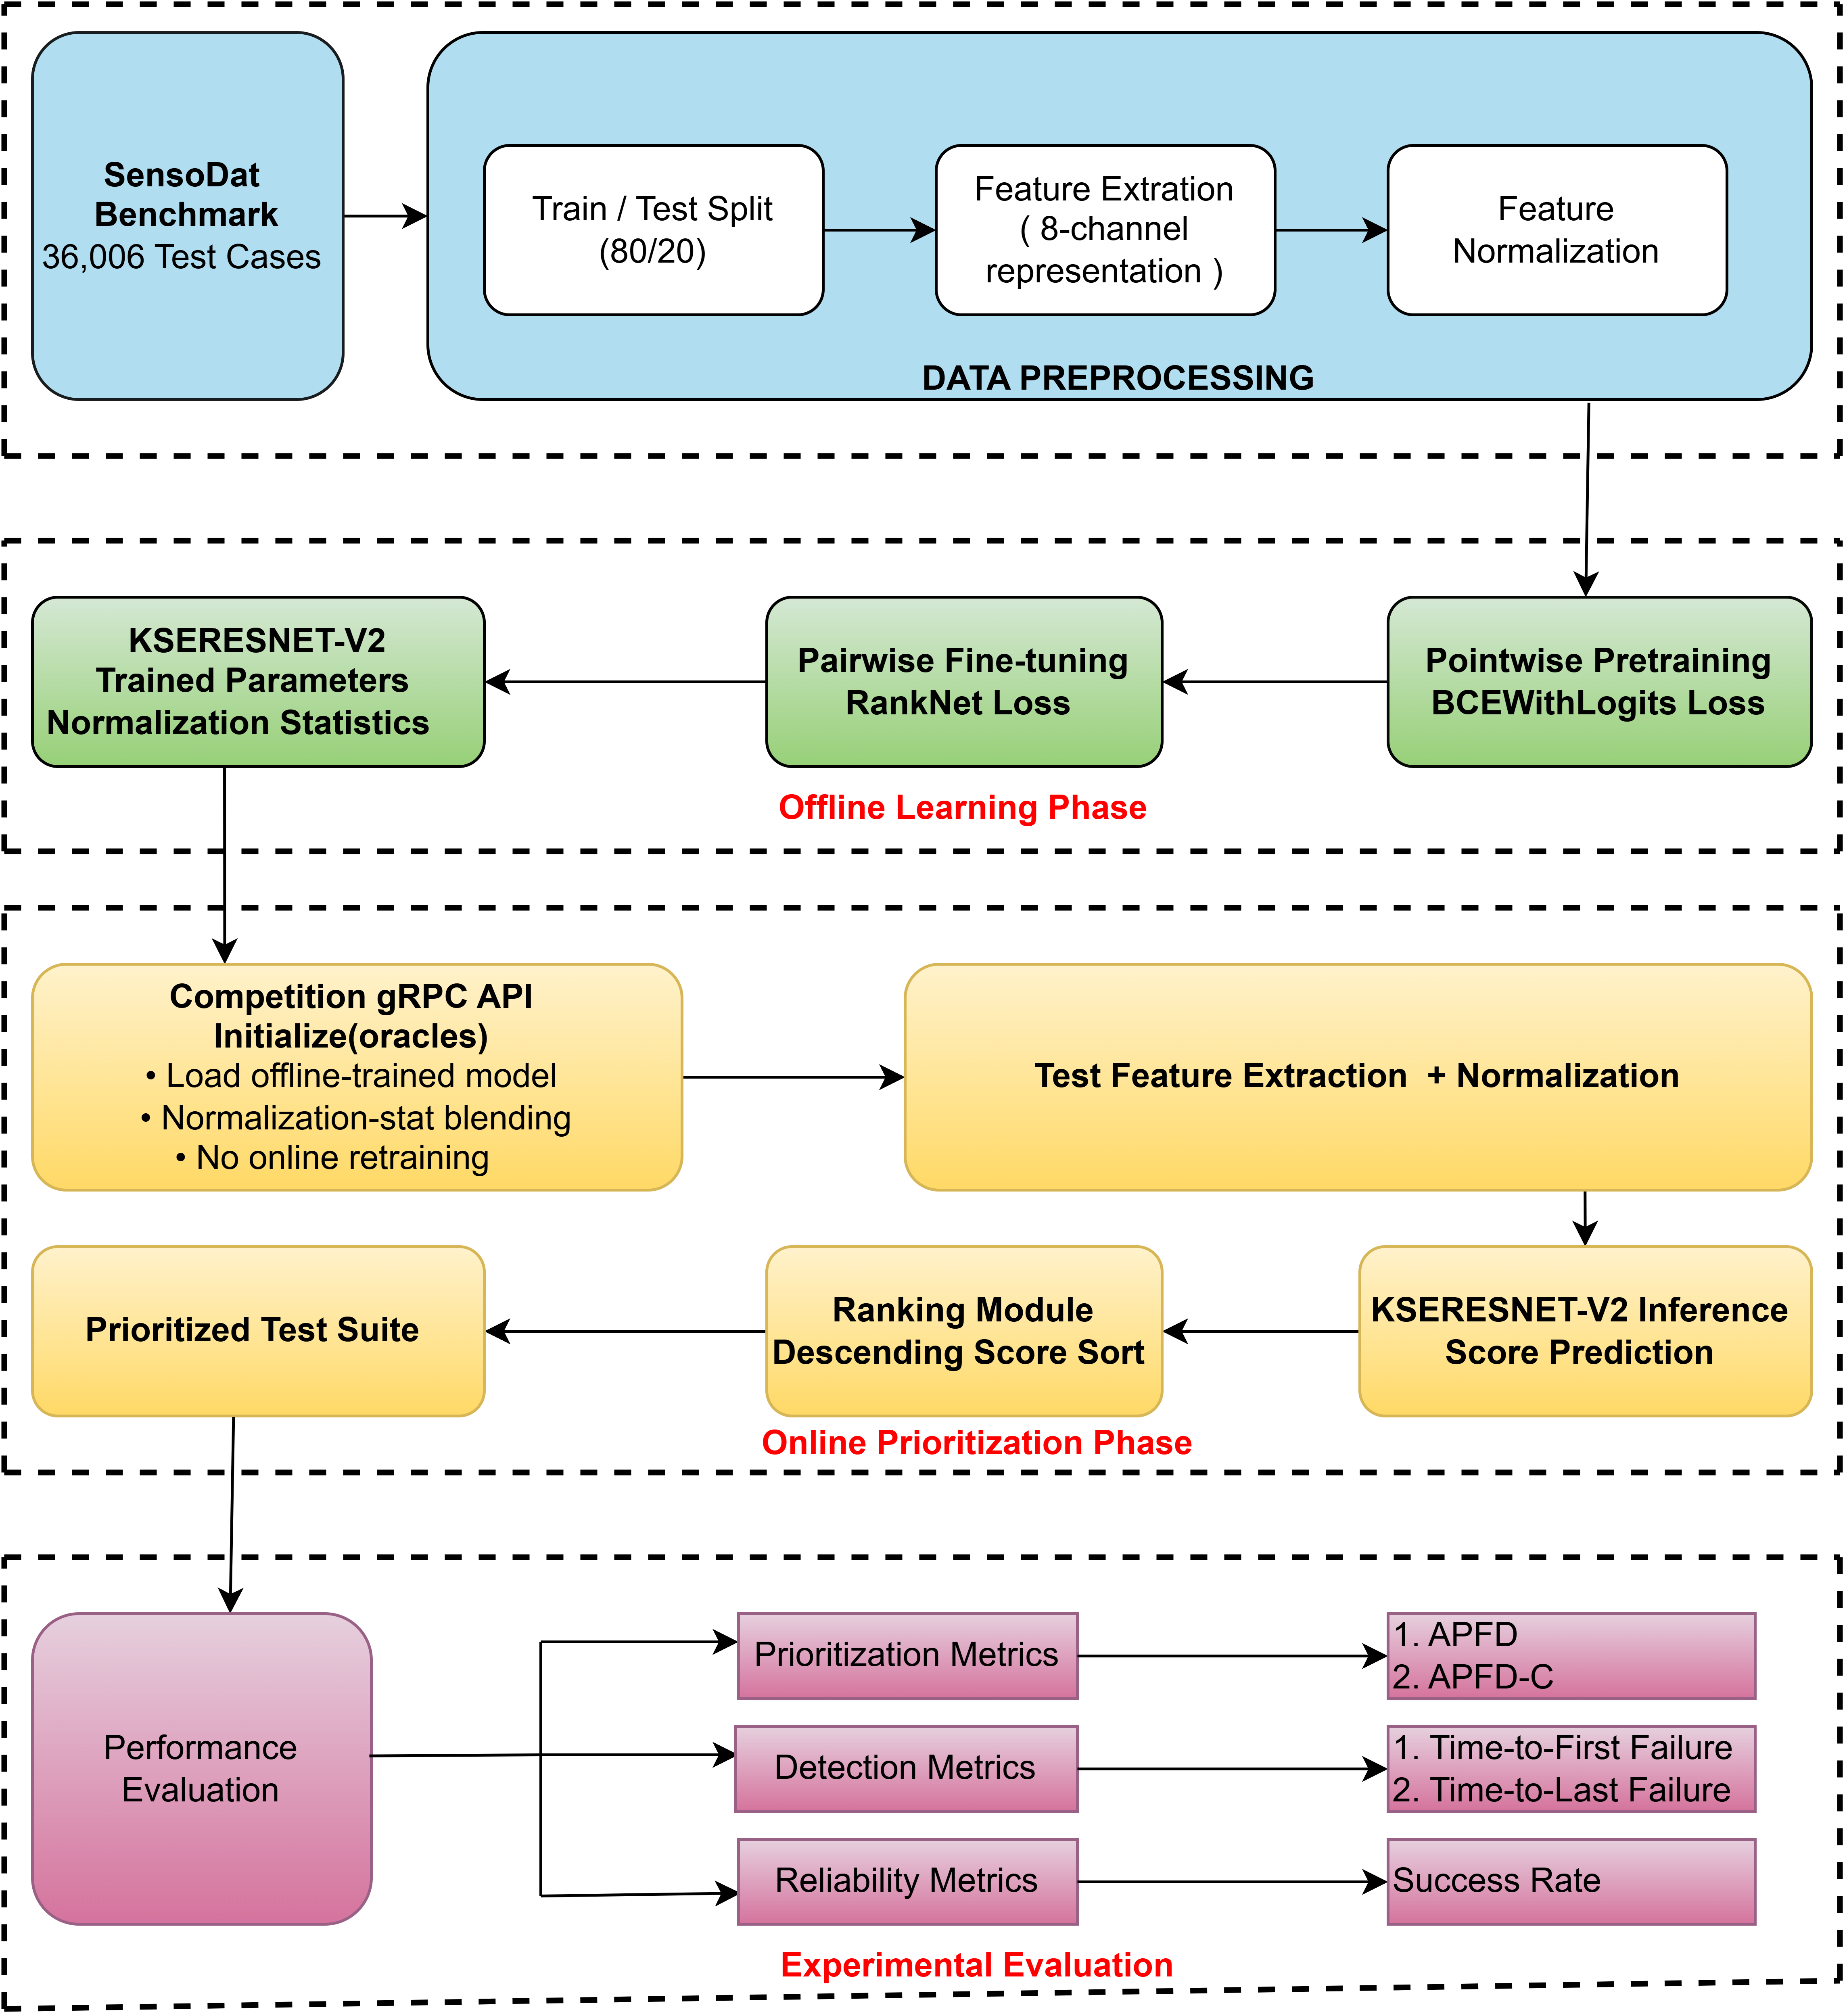
\includegraphics[width=\textwidth]{Fig_Framework.png}
\caption{Framework overview: data preprocessing, offline learning, online
prioritization (via the competition's gRPC interface), and experimental
evaluation.}
\label{fig:framework}
\end{figure}

\textbf{Phase 1 -- Data Preprocessing.} The SensoDat corpus
(Section~\ref{sec:dataset}) is split 80/20 into a training and a held-out
set. Each test case's road waypoints are converted into an 8-channel
feature representation (Section~\ref{sec:proposed}) and normalized.

\textbf{Phase 2 -- Offline Learning.} The model is first pretrained with a
pointwise objective (\texttt{BCEWithLogitsLoss} on pass/fail labels), then
fine-tuned with a pairwise ranking loss (Section~\ref{sec:proposed}) on the
training split only. This phase produces the trained parameters and the
feature-normalization statistics used at inference time -- it happens once,
entirely offline, with full access to the training corpus.

\textbf{Phase 3 -- Online Prioritization.} At evaluation time the model is
driven exclusively through the competition's standardized gRPC interface
(Section~\ref{sec:harness}). \texttt{Initialize(oracles)} loads the
offline-trained parameters and blends the offline normalization statistics
with those observed in the one initialization subject the interface
provides (70\% offline / 30\% observed) -- it does \emph{not} retrain the
model online, a deliberate choice justified by the ablation in
Section~\ref{sec:rq2}. \texttt{Prioritize(tests)} then extracts the same
8-channel features from each unlabeled test, scores it, and sorts
descending by score to produce the prioritized test suite.

\textbf{Phase 4 -- Experimental Evaluation.} The prioritized suite is scored
against three families of metrics: prioritization effectiveness (APFD,
$\mathrm{APFD}_C$), fault-detection speed (time-to-first-failure,
time-to-last-failure), and reliability (success rate) --
Section~\ref{sec:metrics}.

\subsection{Dataset}
\label{sec:dataset}
We use the SensoDat corpus \citep{birchler2024sensodat}, the same dataset
underlying the ICST 2026 competition. We reconstructed the corpus from raw
OpenDRIVE road files and per-test outcome metadata, following the
organizers' own corpus-construction criterion: a test is included only if
both its road definition and its simulator execution trace are present,
i.e., the road was not just generated but successfully executed by the
official pipeline. This yields 32{,}580 unique test cases across three
test generators, matching \citet{aryan2026icst}'s Table~II exactly,
generator-by-generator: 12{,}496 Ambiegen, 12{,}135 Frenetic, and 7{,}949
FreneticV tests. Section~\ref{sec:harness} provides independent
corroborating evidence that this reconstruction is faithful: every one of
the four official tools we did not build ourselves (RoadFury, EagleSemble,
RTE4SDC, ITEP4SDC) reproduces its independently published APFD within 0.03
when run against this corpus, and the two tools with known reliability
defects reproduce the identical root-cause failure. We split the full
32{,}580-test corpus
80/20 (26{,}064 / 6{,}516 tests) with a fixed seed, and used the 20\%
held-out portion \emph{exclusively} for evaluating any model we trained
ourselves, to avoid training/evaluation leakage
\citep{kaufman2012leakage}.

\subsection{Evaluation Harness}
\label{sec:harness}
The organizers' evaluation infrastructure is Docker-based
\citep{boettiger2015introduction}, combined with PostgreSQL and MongoDB,
and not fully self-containable. We re-implemented the evaluation protocol
independently: identical APFD, cost-aware APFD ($\mathrm{APFD}_C$),
time-to-first-fault, and time-to-last-fault formulas
(Section~\ref{sec:metrics}), driving each tool through its standardized
gRPC interface, sampling random subjects (test suites) of a given size,
using one subject for initialization and the remainder for evaluation, as
in \citet{aryan2026icst}. We validated this harness by re-running the four
official 2026 tools and the random baseline and comparing against
\citet{aryan2026icst}'s published Table~III: every tool's measured APFD
matched the published value within 0.03, and both tools with known
reliability issues (EagleSemble, ITEP4SDC) reproduced the identical
root-cause failure (an ONNX runtime type mismatch) at a comparable rate.
This validation is what allows us to treat our own extended experiments
(Sections~\ref{sec:rq2}--\ref{sec:rq4}) as comparable to the organizers'
published baseline figures.

\subsection{Metrics}
\label{sec:metrics}
Given a prioritized order of $n$ tests with $m$ failing tests at positions
$TF_1,\dots,TF_m$, Average Percentage of Fault Detection (APFD)
\citep{rothermel2001prioritizing} is defined as:
\begin{equation}
\mathrm{APFD} = 1 - \frac{\sum_{i=1}^{m} TF_i}{nm} + \frac{1}{2n}
\end{equation}
$\mathrm{APFD}_C$ weights this by each test's simulation cost $C_j$, using
cumulative cost to the $i$-th failure $CF_i$ and total cost $C_{\mathrm{total}}$:
\begin{equation}
\mathrm{APFD}_C = 1 - \frac{\sum_{i=1}^{m} CF_i}{C_{\mathrm{total}} \cdot m} + \frac{1}{2m}
\end{equation}
We additionally report success rate (the proportion of trials producing a
valid, complete ordering) since two competition tools fail on the majority
of runs (Section~\ref{sec:rq1}).

\subsection{Tools Compared}
2026 edition (prioritization): RoadFury \citep{tran2026roadfury},
EagleSemble \citep{aquilinoeaglesemble}, RTE4SDC \citep{maugeri2026rte4sdc},
ITEP4SDC \citep{gullu2026itep4sdc}, a random baseline, our baseline
KSERESNET \citep{swain2026kseresnet}, and our proposed model
(Section~\ref{sec:proposed}). 2025 edition (selection, converted to full
orderings by placing selected tests first and appending the remainder):
CertiFail, Detour, DRVN, ITS4SDC, Curvature-Selector, Graph-Selector,
ML-Selector, and Transformer-Selector.

\subsection{Baseline Model}
KSERESNET \citep{swain2026kseresnet} extracts four kinematic channels from
each test's road waypoints ($\Delta x,\Delta y$ and their second
differences) and scores them with an SE-attention 1D-ResNet
\citep{hu2018squeeze}, trained with pointwise \texttt{BCEWithLogitsLoss} on
pass/fail labels.

\subsection{Proposed Model}
\label{sec:proposed}
Our proposed model retains the baseline's SE-ResNet backbone but (i) extends
the input to eight channels by adding road-geometry features and (ii) is
retrained offline on the full 26{,}064-test training split with a pairwise
ranking loss. Figure~\ref{fig:architecture} details both the feature
derivation and the network itself; we describe each stage below.

\begin{figure}[t]
\centering
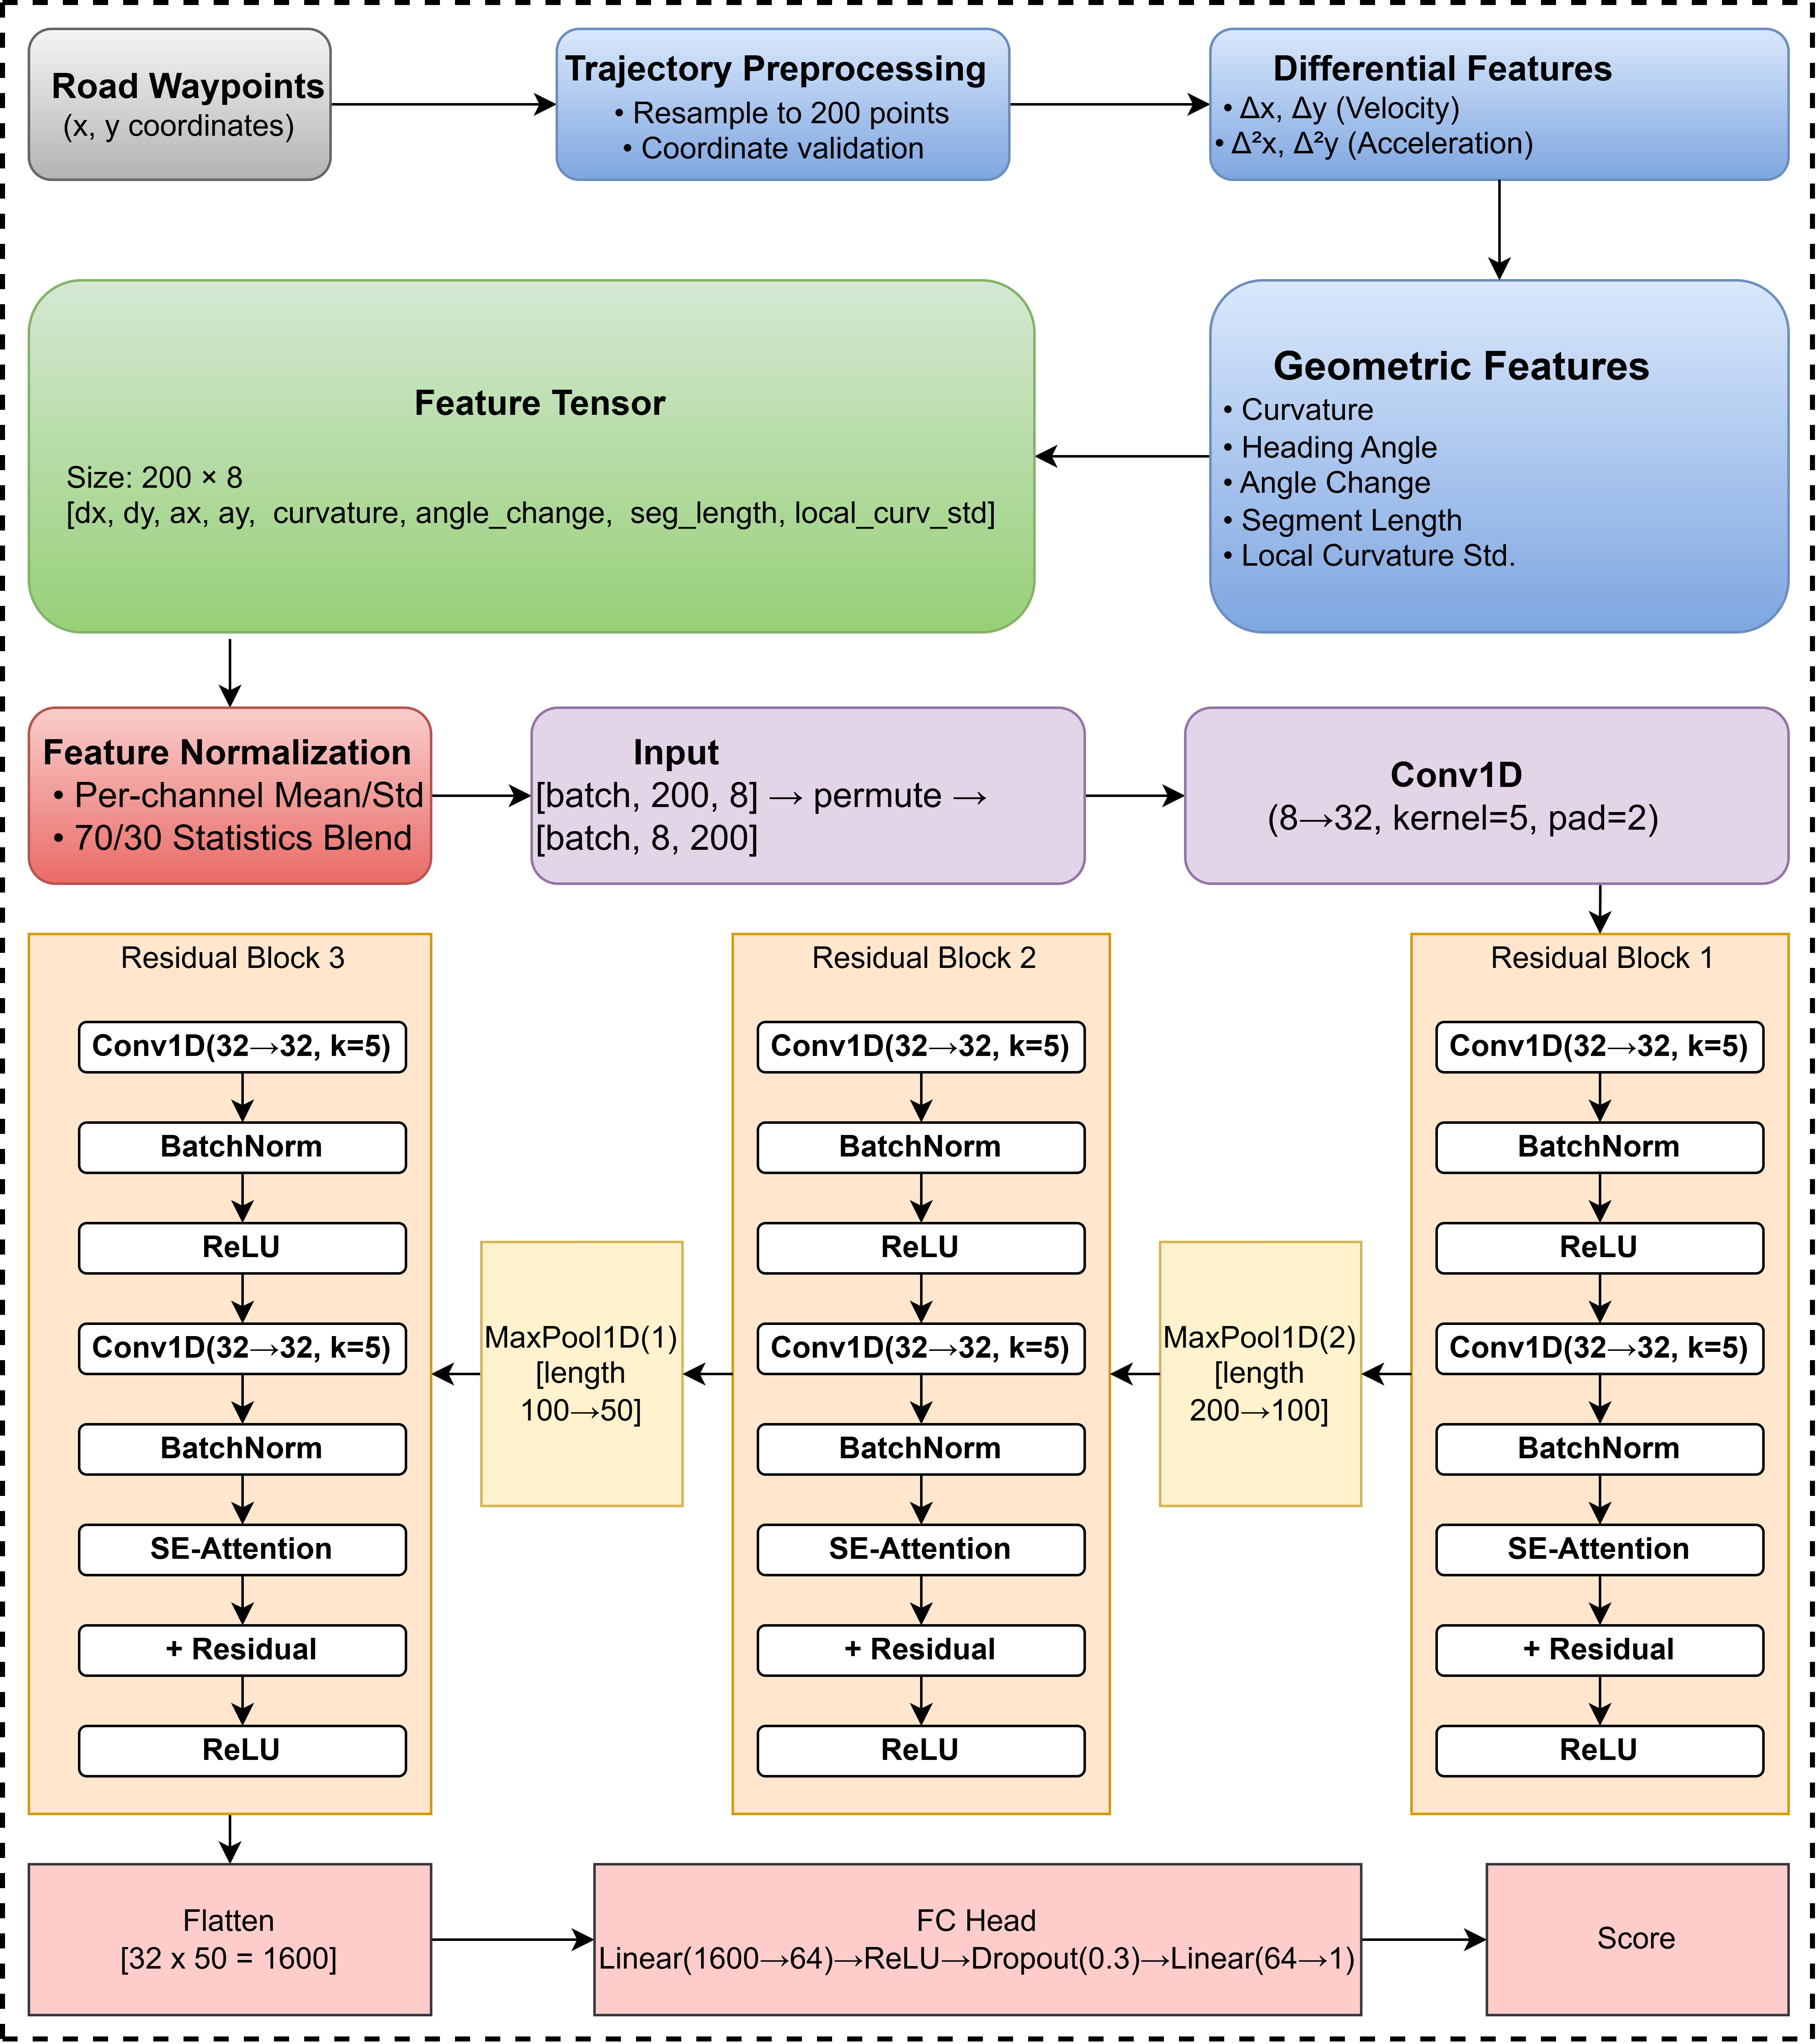
\includegraphics[width=\textwidth]{Fig_Architecture.png}
\caption{Feature extraction and network architecture of the proposed
model. Top: derivation of the 8-channel feature tensor from raw road
waypoints. Bottom: the SE-attention 1D-ResNet that scores the normalized
feature tensor.}
\label{fig:architecture}
\end{figure}

\textbf{Feature derivation (Figure~\ref{fig:architecture}, top).} Raw road
waypoints are resampled/padded to a fixed length of 200 points. Two
feature families are then computed independently from the same
preprocessed trajectory and concatenated: (i) \emph{differential features}
-- $\Delta x,\Delta y$ (first-order displacement) and their second
differences $\Delta^2x,\Delta^2y$ (acceleration), the four channels used by
the baseline model; and (ii) \emph{geometric features}, absent from the
baseline -- segment length $\mathrm{seg\_length}=\sqrt{\Delta x^2+\Delta
y^2}$, heading $\mathrm{atan2}(\Delta y,\Delta x)$, heading angle change
between consecutive segments, curvature (angle change normalized by segment
length), and a local curvature standard deviation over a 5-point window.
The result is an 8-channel, 200-step feature tensor, normalized per-channel
using statistics blended between the offline training set and (at
inference time) the online initialization subject, as described in
Section~\ref{sec:framework}.

\textbf{Network architecture (Figure~\ref{fig:architecture}, bottom).} The
normalized tensor is permuted to $[\text{batch},8,200]$ and passed through
a $1{\times}5$ Conv1D expanding to 32 channels, then three sequential
residual blocks. Each residual block applies two $32{\to}32$, kernel-5
convolutions (each followed by batch normalization \citep{ioffe2015batch}),
a Squeeze-and-Excitation attention gate \citep{hu2018squeeze} that
reweights the 32 channels by a learned, globally-pooled gate, an additive
residual connection, and a final ReLU. A kernel-2 max-pool halves the
sequence length after the first and second residual blocks only
(200$\to$100$\to$50; the third block is followed directly by flattening).
The flattened $32\times50=1{,}600$-dimensional representation is passed
through a fully connected head (Linear(1600$\to$64)$\to$ReLU$\to$Dropout(0.3)
\citep{srivastava2014dropout}$\to$Linear(64$\to$1)) to produce a single
scalar score, with higher scores indicating higher predicted failure risk.

\textbf{Training (offline, Figure~\ref{fig:framework} Phase 2).} The network
is first pretrained with a pointwise objective, then fine-tuned with a
pairwise ranking loss over sampled fail/pass pairs from the training split:
\begin{equation}
\mathcal{L} = \mathrm{E}_{(i,j):\,y_i=\text{FAIL},\,y_j=\text{PASS}}\left[\log\left(1+e^{-(s_i-s_j)}\right)\right]
\end{equation}
where $s_i,s_j$ are model scores for a failing and a passing test,
respectively. The ranking fine-tune warm-starts from the pointwise
checkpoint and trains for 15 epochs over sampled fail/pass pairs
(20{,}000 pairs/epoch) using the Adam optimizer \citep{kingma2014adam};
Section~\ref{sec:rq3-robustness} shows this epoch
count is a genuine optimum, not an arbitrary cutoff. We did not train a
cost-aware variant: the competition's gRPC interface exposes only road
geometry and a binary pass/fail label to the tool at initialization time,
never simulation duration, making $\mathrm{APFD}_C$-aware training
impossible under this interface -- an actionable finding for future
competition editions (Section~\ref{sec:discussion}).

\subsection{Statistical Analysis}
Following established guidance for statistical testing of empirical
software engineering results \citep{arcuri2011practical}, for every paired
comparison we report the mean difference, the Wilcoxon signed-rank test
\citep{wilcoxon1992individual}, and the Vargha--Delaney $\hat{A}_{12}$
effect size \citep{vargha2000critique}, whose conventional magnitude
thresholds we interpret alongside standard effect-size guidance
\citep{cohen2013statistical}. Where multiple tests support a single
research question, we apply a Holm--Bonferroni correction
\citep{holm1979simple} within that family.

\textbf{Unit of analysis.} Every paired test in this paper pairs two tools'
mean APFD on the \emph{same trial} -- a single randomly sampled evaluation
subject (a held-out test suite of a given size) -- not individual test
cases. Both tools in a comparison are scored on an identical, seed-aligned
sequence of subjects, so trial $i$ denotes the same sampled subject for
both. Sample size varies by research question depending on how many trials
were run for that specific comparison: $N=75$ trials (seed 42, subject
sizes 10--80, one trial per size per repeat) for the RQ2 ablation, the
epoch-count and per-generator robustness checks; $N=160$ trials (seed 7,
subject sizes 10--200 across 8 sizes $\times$ 20 repeats) for the RQ3 main
comparisons and the generator-stratified and Transformer robustness
checks. We state $N$ explicitly alongside each test below. Because the
unit of analysis is the trial, not the test case, an extreme p-value
reflects a small $N$ with a highly consistent direction of effect, not a
large sample: e.g., $p=7.6\times10^{-28}$ in RQ3 arises because the
proposed model outperforms the baseline in 159 of the 160 trials with zero
losses (one tie), which drives the paired test close to its theoretical
minimum p-value at that sample size, rather than from any error in $N$.

\textbf{Trial independence.} Because trials are drawn by repeated random
sampling from a shared pool rather than by partitioning it, individual
test cases can appear in more than one trial, which could in principle
correlate trials' outcomes and inflate the Wilcoxon test's apparent
significance. We checked this directly rather than assuming it away, for
both protocols. For the $N=160$ protocol (subject sizes 10--200 drawn from
the 6{,}516-test held-out pool), the mean pairwise Jaccard overlap between
any two trials' evaluation subjects is 0.4\% overall, rising to 2.7\% on
average (6\% at worst, across all 12{,}720 trial pairs) at the largest
subject size (200). For the $N=75$ per-generator protocol (subject sizes
10--80 drawn from smaller, generator-specific pools of 2{,}256--2{,}523
tests), overlap is modestly higher but still small: 0.6--0.7\% overall,
rising to 1.7\% on average (at most 7--8\%, across all 2{,}775 trial
pairs) at the largest subject size (80). Both are expected from the
pool-to-subject size ratio alone and match the organizers' own resampling
protocol \citep{aryan2026icst}: at this scale, cross-trial overlap is not
a material source of correlation, and we treat trials within each
protocol as effectively independent draws.

\section{Results}
\label{sec:results}

\subsection{RQ1: Accuracy Does Not Predict Prioritization Effectiveness}
\label{sec:rq1}
Table~\ref{tab:main} (rows for KSERESNET and Random) shows the baseline
model's independently measured mean APFD is 0.625 -- close to
\citeauthor{aryan2026icst}'s published figure of 0.62 -- against a
self-reported APFD of 0.8131 and a self-reported classification accuracy of
95.27\%. Two distinct gaps are visible here, and it is important not to
conflate them. The first is between the self-reported and independently
measured APFD (0.8131 vs.\ 0.625) -- the \emph{same} metric, measured two
different ways, which we do not diagnose further since we lack access to
the original evaluation code, but which is why every other number in this
paper is drawn exclusively from independently reproduced evaluations
(Section~\ref{sec:harness}). The second, and the one this paper diagnoses
in depth, is between classification accuracy and \emph{any} APFD figure:
even taking the self-reported 0.8131 at face value, 95.27\% accuracy does
not imply near-ceiling ranking performance, and under the independently
measured figure (0.625), it is only 0.11 APFD above a random ordering
(0.513) and 0.18 below the eventual competition winner (0.803). Accuracy
and APFD
are measuring different properties of the model: accuracy rewards correct
pass/fail labels; APFD rewards early placement of failing tests, which a
pointwise-trained model has no explicit incentive to
achieve once its classification boundary is fixed.

\begin{figure*}[t]
\centering
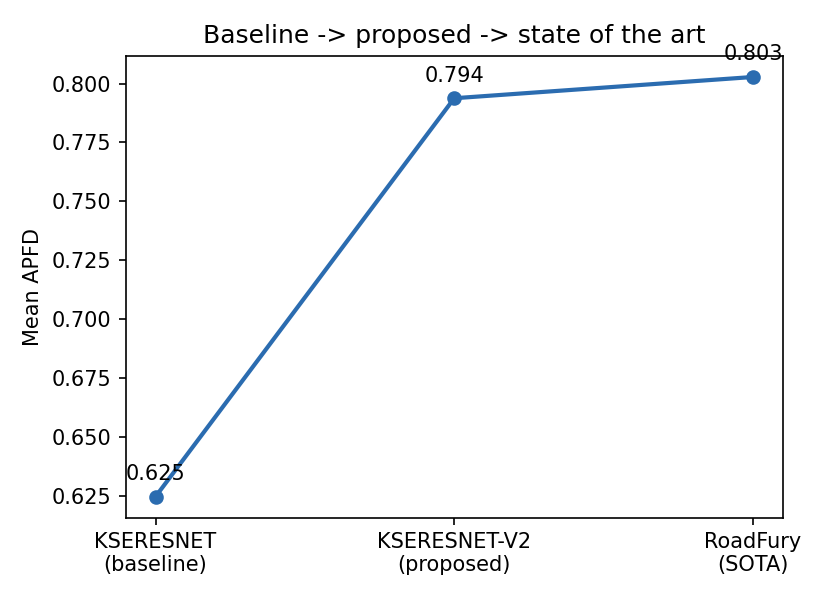
\includegraphics[width=0.8\textwidth]{Fig2.png}
\caption{Mean APFD across the diagnosis-to-remedy trajectory: the
pointwise-trained baseline, our proposed ranking-trained model, and the
competition's state of the art.}
\label{fig:trajectory}
\end{figure*}

Figure~\ref{fig:trajectory} summarizes this trajectory: the baseline sits
far below both the proposed model and the state of the art, despite its
high self-reported classification accuracy.

\subsection{RQ2: Feature Richness, Not Adaptation, Drives Effectiveness}
\label{sec:rq2}
Table~\ref{tab:ablation} reports a $2\times2$ ablation crossing feature set
(baseline 4-channel vs.\ proposed 8-channel) with test-time adaptation
(none vs.\ a pointwise fine-tune on the single subject available at
initialization). This ablation was run on the full 32{,}580-test corpus
(seed 42, subject sizes 10--80, 75 trials) rather than the held-out split
used for the main RQ3 comparison (Table~\ref{tab:main}), since it does not
involve any model we ourselves trained on the training split -- the
baseline's absolute figure here (0.616) is consequently a different sample
from, though consistent with (within 0.009), the 0.625 reported in
Table~\ref{tab:main} under the held-out protocol; both are independent
estimates of the same underlying (untrained-by-us) model's effectiveness,
and their agreement is a sanity check on measurement stability rather than
a claim that the two protocols are interchangeable. Adding the geometry
features while holding adaptation
fixed improves mean APFD by 0.143 ($N=75$ trials, proposed features win 72,
tie 3, lose 0; $\hat{A}_{12}=0.980$, $p=1.7\times10^{-13}$); adding
fine-tuning while holding the feature set fixed improves it by only 0.028
with weak features and, with the richer feature set already in place, is
not merely non-additive but mildly \emph{harmful} ($N=75$ trials,
$\hat{A}_{12}=0.327$, $p=0.022$). Channel-importance analysis
(zeroing each of the 8 channels and measuring the resulting drop in
fail/pass separation AUC \citep{fawcett2006introduction}) confirms the
mechanism: the two geometry channels
absent from the baseline -- heading angle change (AUC drop 0.340) and
curvature (0.272) -- account for the large majority of the model's
discriminative power, while the four original kinematic channels each
contribute less than 0.006. Sharp turns, not raw positional deltas, are
what predict failure in this corpus, which is physically unsurprising but
was not previously quantified for this tool.

\begin{figure}[t]
\centering
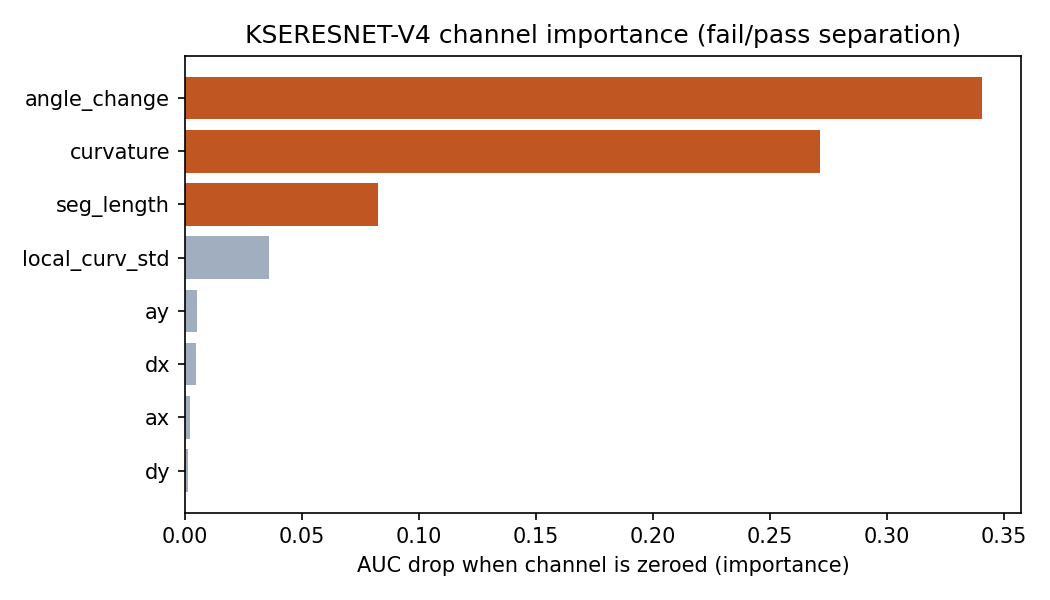
\includegraphics[width=0.8\textwidth]{Fig4.png}
\caption{Channel-importance analysis for the proposed model: AUC drop in
fail/pass separation when each input channel is zeroed. The two geometry
channels absent from the baseline model dominate.}
\label{fig:channels}
\end{figure}

Figure~\ref{fig:channels} shows this ranked by channel.

\subsection{RQ3: A Ranking-Aware Objective Closes Most of the Remaining Gap}
\label{sec:rq3}
Table~\ref{tab:main} reports our main result: retraining with the pairwise
ranking loss (Section~\ref{sec:proposed}) on the held-out split raises mean
APFD from 0.625 to 0.794 ($N=160$ trials, $\hat{A}_{12}=0.997$,
$p=7.6\times10^{-28}$), and $\mathrm{APFD}_C$ from 0.668 to 0.855. As
Section~\ref{sec:methodology} notes, this p-value is extreme because the
effect is extremely consistent, not because $N$ is large: the proposed
model beats the baseline in 159 of these 160 trials, with zero losses and
one tie, so $\hat{A}_{12}=(159+0.5)/160=0.997$ directly reflects that
near-complete pairwise dominance. The proposed model statistically exceeds
RTE4SDC ($N=160$ trials, $\hat{A}_{12}=0.800$, $p=5.9\times10^{-14}$) and is
within 0.009 APFD of RoadFury, the eventual competition winner ($N=160$
trials, $\hat{A}_{12}=0.750$, $p=4.2\times10^{-13}$) -- a real but small
remaining gap. All comparisons survive Holm--Bonferroni correction within
the RQ3 family.

\begin{figure}[t]
\centering
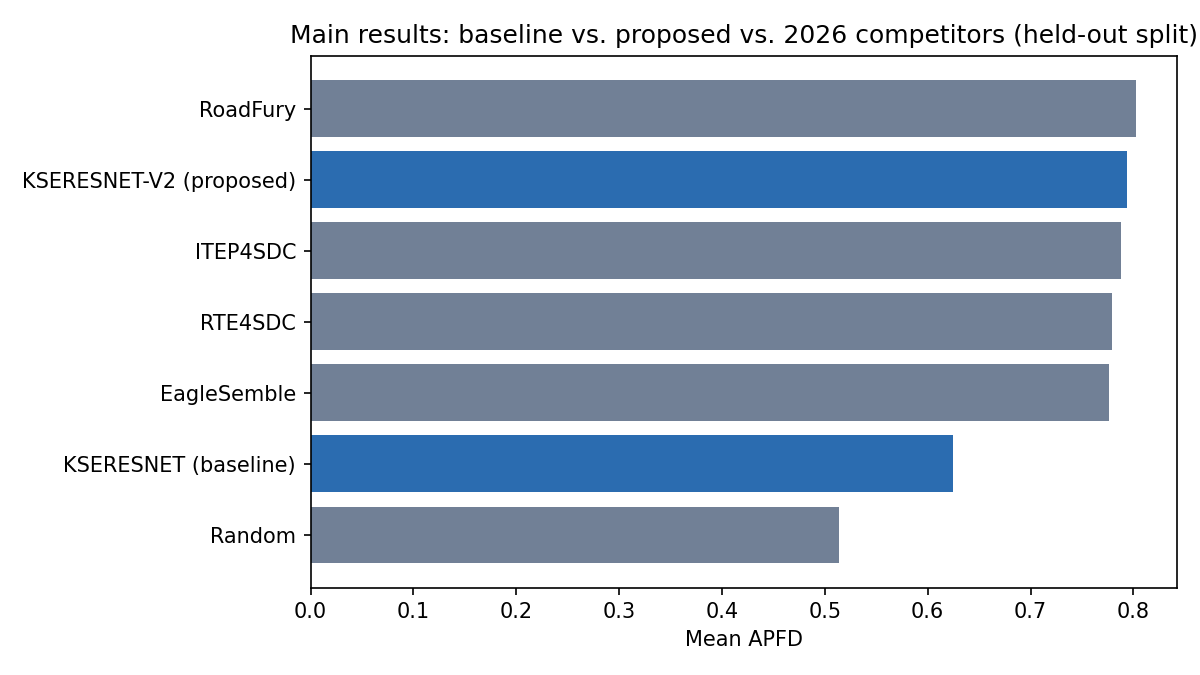
\includegraphics[width=0.8\textwidth]{Fig1.png}
\caption{Mean APFD for all tools compared under the held-out protocol.}
\label{fig:maintools}
\end{figure}

\begin{table}[t]
\caption{Main results: baseline vs.\ proposed vs.\ 2026 competitors,
held-out split (drawn from a pool of 6{,}516 held-out tests; statistical
tests below use $N=160$ trials, subject sizes 10--200).}
\label{tab:main}
\begin{tabular}{lrrrr}
\toprule
Tool & APFD & $\mathrm{APFD}_C$ & Prioritization time (s) & Success rate \\
\midrule
RoadFury \citep{tran2026roadfury} & 0.803 & 0.861 & 0.804 & 100\% \\
\textbf{Proposed (this paper)} & \textbf{0.794} & \textbf{0.855} & 0.370 & \textbf{100\%} \\
ITEP4SDC \citep{gullu2026itep4sdc} & 0.788 & 0.857 & 0.184 & 31\% \\
RTE4SDC \citep{maugeri2026rte4sdc} & 0.779 & 0.836 & 0.244 & 100\% \\
EagleSemble \citep{aquilinoeaglesemble} & 0.777 & 0.851 & 0.477 & 31\% \\
KSERESNET baseline \citep{swain2026kseresnet} & 0.625 & 0.668 & 0.180 & 100\% \\
Random & 0.513 & 0.549 & 0.079 & 100\% \\
\bottomrule
\end{tabular}
\end{table}

\textbf{Why the significance claim is restricted to RTE4SDC.} Table~\ref{tab:main}
shows the proposed model numerically above ITEP4SDC and EagleSemble as well
as RTE4SDC, but we only claim statistical superiority over RTE4SDC, because
ITEP4SDC's and EagleSemble's reported APFD is not computed over a
comparable sample: both succeed on only 31\% of trials, and that success is
not random with respect to difficulty. Breaking their success rate down by
subject size shows a monotonic collapse -- 75\% at size 10, 55\% at size
30, 15\% at size 80, and \emph{0\% at sizes 150 and 200} -- so their
reported APFD is averaged exclusively over the easier, smaller-suite end of
the size range, while RoadFury, RTE4SDC, the proposed model, and Random are
each averaged over the full 10--200 range, including the hardest trials.
This is a survivorship bias, not merely a reliability caveat: it likely
inflates ITEP4SDC's and EagleSemble's reported APFD relative to what they
would score if forced to complete the full trial distribution, and we
therefore treat their figures in Table~\ref{tab:main} as illustrative
rather than as valid heads of a significance comparison. This is discussed
further as a threat to validity in Section~\ref{sec:threats}.

\subsubsection{Robustness checks: four alternative explanations, ruled out}
\label{sec:rq3-robustness}
We tested four plausible alternative paths to closing the remaining gap
to RoadFury (Table~\ref{tab:design}), none of which improved on the main
result. (i) \emph{More training} (40 vs.\ 15 epochs) produced a small but
significant \emph{decrease} ($N=75$ trials, mean APFD $-0.0016$,
$p=0.0003$) -- mild overfitting, not underfitting. (ii)
\emph{Generator-stratified pair sampling} during training, intended to
prevent the model from exploiting cross-generator base failure-rate
differences (Ambiegen 45\% vs.\ Frenetic 37\% vs.\ FreneticV 33\%) rather
than learning genuine within-generator discrimination, produced no
measurable change ($N=160$ trials, $\hat{A}_{12}=0.431$, $p=0.11$), which
also rules out that specific mechanism as an explanation for the RQ4
finding below. (iii) A \emph{Transformer encoder} backbone
\citep{vaswani2017attention}, trained under an identical two-phase
(pointwise pretrain, then ranking fine-tune) recipe on the same features,
performed substantially \emph{worse} than the ResNet ($N=160$ trials,
mean APFD 0.742 vs.\ 0.794, the ResNet wins 148 of 160 trials with 4
losses and 8 ties; $\hat{A}_{12}=0.050$, $p<10^{-25}$) -- architecture
family is not, on this budget, a lever toward closing the gap, even though
the competition's best-performing tool (RoadFury) also uses a Transformer,
which we attribute to differences in feature richness or training scale we
did not have access to reproduce, not to the architecture per se. (iv) A
\emph{listwise} ranking loss (ListNet-style top-1 cross-entropy
\citep{cao2007learning}, computed over randomly sampled 32-item lists
rather than fail/pass pairs, same warm-start and training split as the
proposed model) performed substantially \emph{worse} than the pairwise
loss used in the proposed model ($N=160$ trials, mean APFD 0.772 vs.\
0.794, the pairwise-trained model wins 136 of 160 trials with 7 losses
and 17 ties; $\hat{A}_{12}=0.097$, $p=9.8\times10^{-23}$) -- for this
architecture, feature set, and training budget, the pairwise objective is
not merely a reasonable default but the better-performing of the two
ranking formulations we tested.

\begin{table}[t]
\caption{Alternative design choices tested and not adopted. Unit of
analysis is the trial (Section~\ref{sec:methodology}): $N=75$ trials for
the epoch-count row, $N=160$ trials for the other three. $\hat{A}_{12}$ is
$P(\text{alternative} > \text{proposed})$ throughout, matching the sign of
the mean-difference column; values below 0.5 indicate the proposed model
wins more often.}
\label{tab:design}
\begin{tabular}{p{2.7cm}p{3.0cm}p{1.3cm}p{2.3cm}}
\toprule
Design choice & Result vs. proposed model & $\hat{A}_{12}$ & Decision \\
\midrule
More training epochs (40 vs. 15) & $-0.0016$ APFD, $p=0.0003$ & 0.373 & Not adopted -- mild overfitting \\
Generator-stratified pair sampling & $-0.0004$ APFD, $p=0.11$ (n.s.) & 0.431 & Not adopted -- no effect \\
Transformer backbone (same recipe) & $-0.052$ APFD, $p<10^{-25}$ & 0.050 & Not adopted -- underperforms ResNet \\
Listwise ranking loss (ListNet-style, same recipe) & $-0.0214$ APFD, $p=9.8\times10^{-23}$ & 0.097 & Not adopted -- underperforms pairwise loss \\
\bottomrule
\end{tabular}
\end{table}

\subsection{RQ4: Aggregate Improvement Masks Generator-Level Regressions}
\label{sec:rq4}
Breaking the RQ3 comparison down by road generator (Table~\ref{tab:gen})
reveals that the proposed model's aggregate improvement is not uniform.
Relative to the intermediate, pointwise-trained, feature-only model (the
same condition as ``Proposed features + pointwise fine-tune'' in
Table~\ref{tab:ablation}, here resampled per generator under a separate
held-out protocol of $N=75$ trials per generator, seed 42, subject sizes
10--80), the proposed (ranking-trained) model is significantly
\emph{worse} on Ambiegen (loses 42 of 75 trials, wins 20, ties 13;
$\hat{A}_{12}=0.353$, $p=0.003$) and FreneticV (loses 43 of 75, wins 6,
ties 26; $\hat{A}_{12}=0.253$, $p<0.0001$), and not significantly
different on Frenetic (wins 26, ties 24, losses 25; $p=0.28$). In raw APFD
these regressions are small (0.004 and 0.008 respectively); we report the
effect size alongside the p-value, rather than the p-value alone, because
$\hat{A}_{12}$ is what shows these are a consistent shift in outcome across
most of the 75 trials rather than a large swing in a handful of them:
$\hat{A}_{12}=0.253$ and $0.353$ both fall at or beyond the conventional
medium-to-large threshold for the Vargha--Delaney statistic
\citep{vargha2000critique}. We report this as a real but modest finding:
it is not, on its own, grounds to prefer the intermediate model in
practice, but it does mean the aggregate RQ3 improvement should not be
read as a uniform within-generator improvement.
This is a Simpson's-paradox-like effect \citep{simpson1951interpretation}: the
aggregate, mixed-generator comparison shows improvement because it also
rewards correctly ordering \emph{across} generators with different base
failure rates, which the ranking loss appears to partly learn, but this
does not correspond to uniformly better \emph{within}-generator ranking.
The generator-stratified robustness check (Section~\ref{sec:rq3-robustness})
shows this is not fixed by stratifying training pairs by generator, so the
mechanism is not simply an artifact of pair-sampling imbalance. The
listwise robustness check (Section~\ref{sec:rq3-robustness}) shows the
pattern is not specific to the pairwise loss either, but it is not
identical under a different objective: relative to the same intermediate
model, the listwise-trained model ($N=75$ trials per generator) regresses
significantly on Frenetic (loses 46 of 75, wins 28, ties 1;
$\hat{A}_{12}=0.380$, $p=0.005$) and FreneticV (loses 50 of 75, wins 22,
ties 3; $\hat{A}_{12}=0.313$, $p<0.001$), but \emph{not} on Ambiegen (loses
45 of 75, wins 29, ties 1; $p=0.15$, n.s.) -- the reverse of the pairwise
model's pattern, which regresses on Ambiegen and FreneticV but not
Frenetic. Some generator-level regression recurs under both ranking
objectives, but which generator it appears on is not stable across them,
which argues against a single fixed root cause (e.g., one generator's
roads being intrinsically harder to rank) and toward each objective
learning a somewhat different, imperfect approximation of the true
ranking. To our
knowledge, no prior evaluation of ML-based SDC test prioritizers reports a
per-generator breakdown; aggregate APFD alone would not have surfaced this.

\begin{figure}[t]
\centering
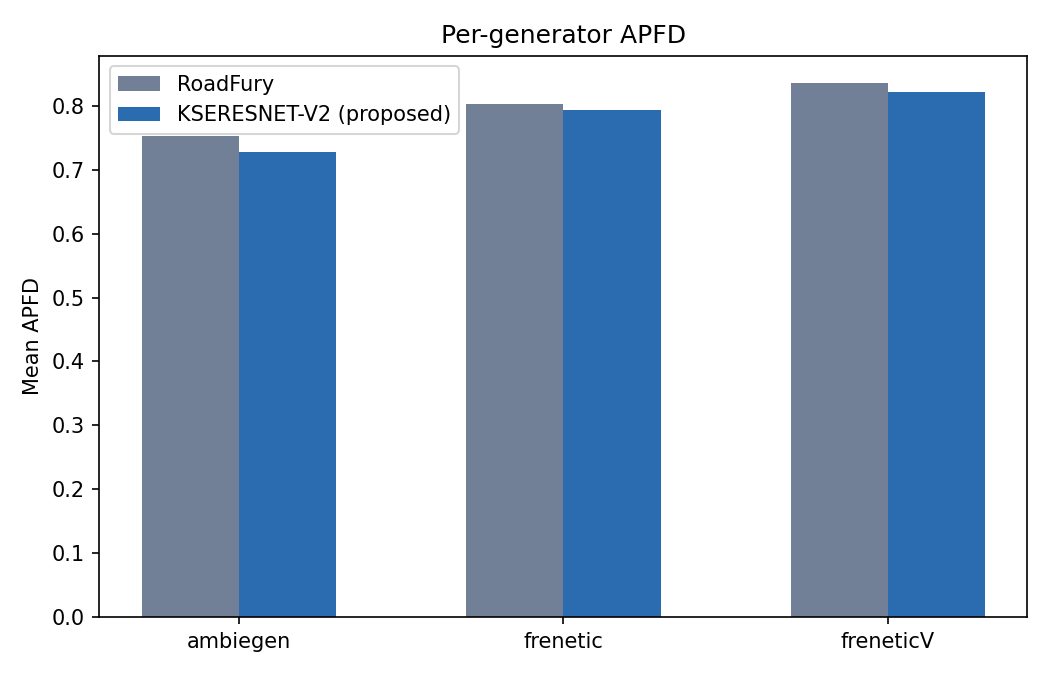
\includegraphics[width=0.8\textwidth]{Fig3.png}
\caption{Per-generator mean APFD: RoadFury vs.\ the proposed model. The
aggregate advantage narrows or reverses within individual generators.}
\label{fig:pergen}
\end{figure}

\begin{table}[t]
\caption{Per-generator APFD (mean), $N=75$ trials per generator (seed 42,
subject sizes 10--80).}
\label{tab:gen}
\begin{tabular}{lrrr}
\toprule
Generator & RoadFury & Feature-only (intermediate) & Proposed \\
\midrule
Ambiegen & 0.753 & 0.732 & 0.728 \\
Frenetic & 0.803 & 0.792 & 0.794 \\
FreneticV & 0.836 & 0.830 & 0.822 \\
\bottomrule
\end{tabular}
\end{table}

A test-count-weighted average of Table~\ref{tab:gen}'s three rows will
\emph{not} reproduce Table~\ref{tab:main}'s aggregate figures (e.g., for
the proposed model, roughly 0.78 versus 0.794): the two tables use
different sampling schemes, not just different weights. Table~\ref{tab:gen}
subjects are drawn purely from within a single generator's own subpool and
capped at subject size 80, whereas Table~\ref{tab:main}'s subjects are
drawn from the full, mixed-generator held-out pool across sizes 10--200,
including sizes (100--200) absent from the per-generator breakdown
entirely. This is not an inconsistency to reconcile away -- it is the same
distinction RQ4 turns on: mixed-generator subjects reward correctly
ordering \emph{across} generators, which pure single-generator subjects
structurally cannot reward, so the two tables are measuring related but
not arithmetically interchangeable quantities.

\subsection{RQ5: Selection Tools Underperform When Converted to Prioritizers}
\label{sec:rq5}
Every converted 2025 selection tool scores below the proposed model, and
six of the seven score below even the pointwise baseline
(Table~\ref{tab:crossedition}): best is ITS4SDC (0.707), worst is Detour
(0.520). This is consistent with task-specific design mattering: a model
trained to identify a good \emph{subset} has no training signal for
ordering the remainder of the suite, which our conversion procedure fills
with an uninformative random order.

\begin{table}[t]
\caption{2025 selection tools converted to full orderings (full corpus).}
\label{tab:crossedition}
\begin{tabular}{lrr}
\toprule
Tool & APFD & Success rate \\
\midrule
ITS4SDC & 0.707 & 100\% \\
Curvature-Selector & 0.597 & 100\% \\
Graph-Selector & 0.587 & 100\% \\
Transformer-Selector & 0.560 & 100\% \\
CertiFail & 0.549 & 100\% \\
ML-Selector & 0.546 & 100\% \\
DRVN & 0.537 & 99\% \\
Detour & 0.520 & 99\% \\
\bottomrule
\end{tabular}
\end{table}

\begin{table}[t]
\caption{Ablation: feature set $\times$ adaptation strategy. $N=75$ trials
(seed 42, subject sizes 10--80) per cell.}
\label{tab:ablation}
\begin{tabular}{lrr}
\toprule
Configuration & Mean APFD & Std. \\
\midrule
Baseline features, no adaptation & 0.616 & 0.061 \\
Baseline features + pointwise fine-tune & 0.644 & 0.074 \\
Proposed features, no adaptation & 0.759 & 0.054 \\
Proposed features + pointwise fine-tune & 0.758 & 0.056 \\
\bottomrule
\end{tabular}
\end{table}

\section{Discussion}
\label{sec:discussion}
\textbf{For practitioners building ML-based SDC prioritizers}: invest in
domain-informed feature engineering before investing in training-objective
sophistication or architecture search -- in this study, features accounted
for roughly five times the effect size of either. \textbf{For competition
organizers}: the gRPC interface used in this and the prior edition does not
expose simulation cost to the tool at initialization time, which makes
genuine $\mathrm{APFD}_C$-aware training structurally impossible; exposing
cost (even approximately) would let future submissions target the metric
they are actually scored on. \textbf{For evaluators of this class of tool
generally}: our RQ4 finding argues for reporting per-subgroup breakdowns
(by generator, by scenario type, etc.) alongside aggregate metrics, since
an aggregate improvement is not guaranteed to generalize within any given
subgroup.

\section{Threats to Validity}
\label{sec:threats}
We organize this section using the construct/internal/external/conclusion
validity framework of \citet{wohlin2012experimentation}, consistent with
current empirical software engineering reporting standards
\citep{ralph2020empirical}.
\textbf{Construct.} APFD is a standard but imperfect proxy for
fault-detection cost-effectiveness; we also report $\mathrm{APFD}_C$ where
possible. \textbf{Internal.} We
do not control how the original KSERESNET checkpoint was trained or on what
data; our own proposed model's evaluation is protected from this specific
threat by the leakage-free 80/20 split, but
the baseline's absolute number should be read as "what the organizers
independently measured," not "what we can vouch for the training
process of." Our CPU-only training budget may understate what a
Transformer backbone (Section~\ref{sec:rq3-robustness}) could achieve with
more compute; we report this as a bounded, not universal, negative result.
Similarly, our listwise check (Section~\ref{sec:rq3-robustness}) tests one
specific formulation (ListNet-style top-1 cross-entropy over 32-item
lists) and does not rule out that a different listwise loss, list size, or
training budget (e.g., LambdaRank's NDCG-weighted gradients) could close
the gap to the pairwise loss; we report the negative result for the
formulation we tested, not for listwise objectives in general.
A more consequential internal threat is \emph{survivorship bias} in the
ITEP4SDC and EagleSemble comparisons: both succeed on only 31\% of trials,
and their successes are concentrated at smaller, easier subject sizes
(Section~\ref{sec:rq3}), so their reported APFD is not computed over a
sample comparable to the fully reliable tools. This kind of
size-/difficulty-dependent failure is consistent with broader findings on
non-deterministic, environment-sensitive test behavior
\citep{luo2014empirical} and on the gap between reported and
production-grade reliability of deployed ML components
\citep{sculley2015hidden}. We mitigate this by
restricting our significance claims to RTE4SDC, but the numeric comparisons
against ITEP4SDC and EagleSemble elsewhere in this paper (e.g.,
Table~\ref{tab:main}) should be read as descriptive, not as validated
head-to-head claims. Relatedly, the per-generator regressions reported in
RQ4 are small in absolute APFD terms (0.004--0.008); we report them because
their Vargha--Delaney effect sizes ($\hat{A}_{12}=0.253$--$0.353$, $N=75$
trials per generator) show the proposed model losing a majority of
individual trials to the intermediate model in Ambiegen and FreneticV, not
because $p<0.05$ makes the difference notable on its own -- but we do not
claim these regressions are large enough to change a practitioner's tool
choice on their own. \textbf{External.} All experiments use a single
dataset (SensoDat) and a single simulator; we did not replicate any of
RQ1--RQ4 on a second corpus, and this is a real limitation, not a merely
disclosed one. We did not attempt a second corpus in this revision because
a faithful replication is not a small addition: it requires a simulator
producing comparable road-geometry test artifacts with ground-truth
pass/fail outcomes (e.g., a BeamNG.tech-based generator
\citep{papamichail2025scenario} or a CARLA-based scenario suite), a
harness re-validated against that simulator's own published baselines the
way we validated ours against \citet{aryan2026icst}'s Table~III
(Section~\ref{sec:harness}), and a leakage-free retraining of both the
baseline and proposed model on that corpus -- in effect, most of this
paper's methodology repeated end to end. This is also why we frame RQ1's
central finding at the level of a training-objective mismatch (pointwise
loss optimized, ranking metric scored) rather than at the level of
SensoDat-specific data properties: the mismatch follows from a
general learning-to-rank argument \citep{burges2005learning} that does not
reference SensoDat, which is why we expect it to recur elsewhere, but this
is a theoretical argument for external validity, not an empirical one, and
we do not present it as a substitute for a second-corpus replication. We
single out RQ4 (the per-generator regression) as the finding least likely
to generalize as stated, since it is defined in terms of SensoDat's three
specific generators; a second corpus would show whether \emph{some}
generator-level regression recurs, not whether these same three do.
Cross-corpus replication is the most valuable single follow-up to this
paper, and we leave it as future work rather than an in-scope contribution.
\textbf{Conclusion validity.} We apply
Holm--Bonferroni correction within each RQ's family of tests to mitigate
multiple-comparison risk.

\section{Conclusion and Future Work}
Classification accuracy is not a reliable proxy for prioritization
effectiveness in ML-based SDC test prioritization: 95.27\% self-reported
accuracy corresponded to an independently measured mean APFD of only 0.625,
just 0.11 above a random ordering. This effect is diagnosable (a pointwise
training objective) and substantially repairable (a ranking-aware
retraining closes the gap to the state of the art from 0.18 to 0.009 APFD)
without discarding the underlying architecture. This repair is not,
however, complete or uniform: two of three generators show a small but
statistically consistent regression under a per-generator breakdown, and
four plausible follow-up improvements (more training, stratified
sampling, a Transformer backbone, a listwise ranking loss)
did not close the remaining gap further. Future work should pursue a full
(not warm-started) retraining of the base model, address the
generator-level regression directly, and, if competition infrastructure is
extended to expose simulation cost, pursue genuinely cost-aware training.
The single highest-priority follow-up, however, is replicating RQ1--RQ4 on
a second SDC corpus and simulator (Section~\ref{sec:threats}), since every
finding in this paper is currently established on SensoDat alone.

\section*{Statements and Declarations}
\textbf{Funding.} This work is supported by DIAL Grant, IBITF, IIT Bhilai,
DST, Govt. of India.
\textbf{Competing interests.} The authors declare no competing interests.
\textbf{Data availability.} The SensoDat corpus is publicly available
\citep{birchler2024sensodat}. All code, trained model checkpoints, dataset
splits, and the independent evaluation harness used in this paper are
released at \url{https://github.com/VishalKumarSwain/kseresnet-v2-artifact}
(archived on Zenodo: \url{https://doi.org/10.5281/zenodo.21273306}).
\label{sec:availability}

\bibliographystyle{spbasic}
\bibliography{references}

\end{document}
